\documentclass[a4paper, twoside]{article}
\usepackage[margin=12mm, bottom=0.75in, verbose]{geometry}
\usepackage{graphicx}
\usepackage{here, multicol, fancyhdr}
\usepackage{charter, courier}
\usepackage[OT1,T1]{fontenc} %use TeX encoding then Type 1.
\usepackage[protrusion=true, expansion=true]{microtype} % Better typography
\usepackage[english]{babel} % English language/hyphenation
\usepackage[utf8]{inputenc}
\usepackage{amsmath,amsfonts,amsthm} % Math packages
\usepackage{lettrine} % dropped capital letter
\usepackage{booktabs} % Horizontal rules in tables
\usepackage[small, labelfont=bf, up, textfont=up]{caption}
\usepackage[rgb]{xcolor} % Should be CMYK if supported by the system

% Colours by PRACE graphics guidelines
%\definecolor{prace-darkblue}{rgb}{0.1, 0.19, 0.48} % 25, 49, 123
%\definecolor{prace-lightblue}{rgb}{0.52, 0.81, 0.94} %132, 206, 239
% Colours by SoHPC logo pipette measurements
\definecolor{prace-orange}{rgb}{1.0,0.42, 0.1} % 255, 107, 25
\definecolor{prace-darkblue}{rgb}{0.08, 0.31, 0.58} % #155195 = 21,81,149
\definecolor{prace-lightblue}{rgb}{0.32, 0.73, 0.93} % #51bbed = 81,187,237
\newcommand{\highlight}[1]{\textcolor{prace-orange}{#1}}
\definecolor{link}{rgb}{0.1, 0.19, 0.48}

\usepackage{sectsty} % Enables custom section titles
\allsectionsfont{\large\color{prace-orange}\usefont{OT1}{phv}{m}{n}}
\usepackage[superscript,biblabel]{cite}
\usepackage{calc,float,wrapfig}\restylefloat{figure}

\usepackage[colorlinks=true, linkcolor=link, anchorcolor=link,citecolor=link,
filecolor=link, menucolor=link,urlcolor=prace-darkblue]{hyperref}

%\pagestyle{empty}
% Do not enable page numbering below as it will be inserted by the publication
%\pagestyle{fancy}\fancyhf{}\renewcommand{\headrulewidth}{0pt}\renewcommand{\footrulewidth}{0pt}\fancyfoot[C]{\colorbox{orange}{\raisebox{0mm}[4mm][7mm]{\textcolor{white}{\usefont{OT1}{phv}{m}{n}\selectfont~\thepage~}}}}
%To automatically convert Inkscape SVG into PDF or EPS use:
% pdflatex -synctex=1  --enable-write1 sohpc-template.tex
\newcommand{\includegraphicsvg}[2][]{%
  \ifnum\pdfstrcmp{\pdffilemoddate{./#2.svg}}%
  {\pdffilemoddate{../gen/#2.pdf}}>0%
  {\immediate\write18{inkscape -z -D --file=./#2.svg %
      --export-pdf=#2.pdf --export-eps=#2.eps %
      --export-area-drawing}}\fi%
  \includegraphics[#1]{#2}%
}

\newcommand{\itempar}[1]{\noindent\highlight{\textsf #1}\par\noindent}

\graphicspath{{img/}}

% http://tex.stackexchange.com/questions/59166/span-column-in-a-multicols-environment
%\newcounter{tempcolnum}
%\makeatletter
%\newcommand{\multicolinterrupt}[1]{% Stuff to span rows
%\setcounter{tempcolnum}{\col@number}
%\end{multicols}
%#1%
%\begin{multicols}{\value{tempcolnum}}
%}
%\makeatother

\hyphenation{SoHPC AntiSpam} % do not hyphenate

\usepackage{titling}


\pretitle{\vspace{-30pt} \begin{flushleft}
    \usefont{OT1}{phv}{m}{n}\selectfont\large}

\title{Web Visualisation of Energy Load of an HPC System} % Your article title

\posttitle{\par \end{flushleft} \vskip 0.5ex}

\renewcommand{\maketitlehookb}{\par\noindent\flushleft%
\fontsize{45}{50}\usefont{OT1}{phv}{m}{n}\selectfont%
\highlight{Visualising} HPC System's Load}

\preauthor{\vskip 0.9ex \begin{flushleft}\large
    \usefont{OT1}{phv}{b}{sl} \color{prace-orange}}

\author{Petr Stehl\'ik} % Name and surname

\postauthor{\par\end{flushleft}}

\predate{}\date{}\postdate{\vspace{-50pt}}

% Do not enable fancy pagestyle as it will be used at booklet composition.
\fancypagestyle{plain}{\fancyhf{}\renewcommand{\headrulewidth}{0pt}\renewcommand{\footrulewidth}{0pt}\fancyfoot[C]{\colorbox{orange}{\raisebox{0mm}[4mm][7mm]{\textcolor{white}{\usefont{OT1}{phv}{m}{n}\selectfont~\thepage~}}}}}
\pagestyle{plain}
\pagestyle{empty}
\begin{document}
\noindent
\begin{minipage}{0.55\linewidth}
  \maketitle
  \fontsize{14pt}{20pt}\usefont{OT1}{phv}{m}{n}\selectfont
  \raggedright
    Energy efficiency is one of the most timely problems in managing HPC facilities which can be addressed at different scale and perspective. Using Internet of Things technologies this project focuses on visualising data collected from the Galileo supercomputer in a web application.
  \end{minipage}\hfill
\begin{minipage}{0.40\textwidth}
  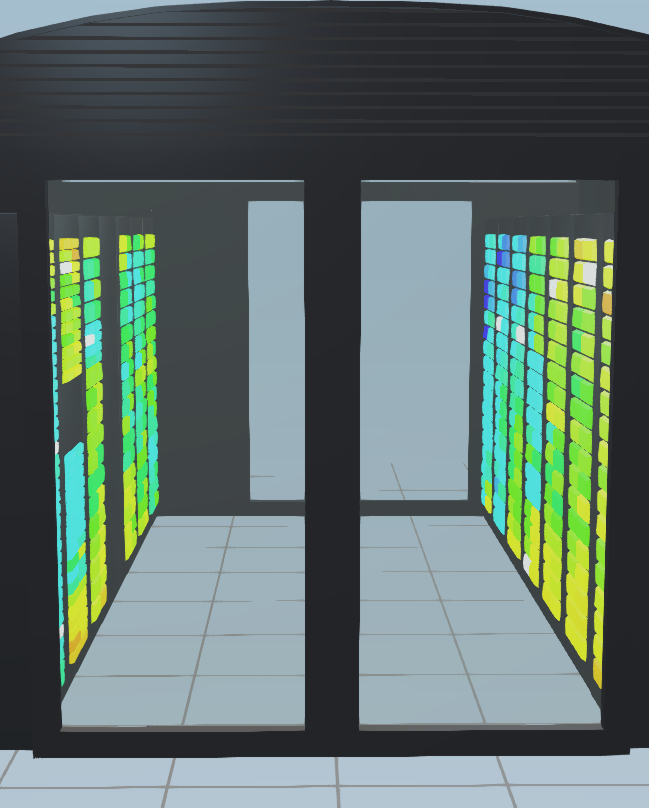
\includegraphics[width=\linewidth]{3d-model}
  %\includegraphicsvg[width=\linewidth]{sohpc-logo}
  \thispagestyle{empty}
\end{minipage}
\vskip 30pt
\frenchspacing
\begin{multicols}{3}

\lettrine[lines=4,nindent=0em]{\highlight{T}}{}he current monitoring system\cite{current} consists of several layers which allow to aggregate in a single point heterogeneous data sources which consist of computing elements, node, job scheduler and facility telemetry of the Galileo supercomputer located at CINECA, Bologna, Italy.

The system was named \textit{ExaMon}\footnote{Shorthand for Exascale Monitoring} and is built on top of MQTT protocol\cite{mqtt} which allows measured metrics to be send to a central broker where received data are processed and stored in KairosDB\cite{kairos} database utilizing Cassandra cluster.

\begin{figure}[H]
%\color{yellow}\rule{\linewidth}{3cm}\color{black}
    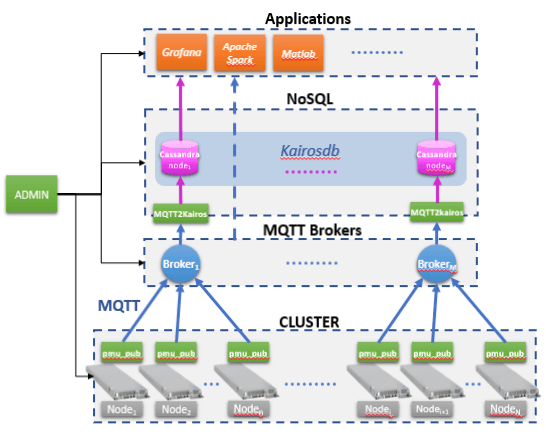
\includegraphics[width=0.9\linewidth]{examon-architecture}
    \caption{Examon Architecture}
    \label{arch}
\end{figure}

This enables us to post-process data in time-oriented fashion in order to visualise them on a time-line and as a single number as well.

Current implementation uses Grafana framework to visualise data stored in KairosDB. Grafana will be replaced by the project's result of creating a dedicated web application for defined use-cases with 3D model of a cluster room showing various metrics of the whole HPC system with focus on energy consumption and efficiency.

\begin{figure*}[b!]
    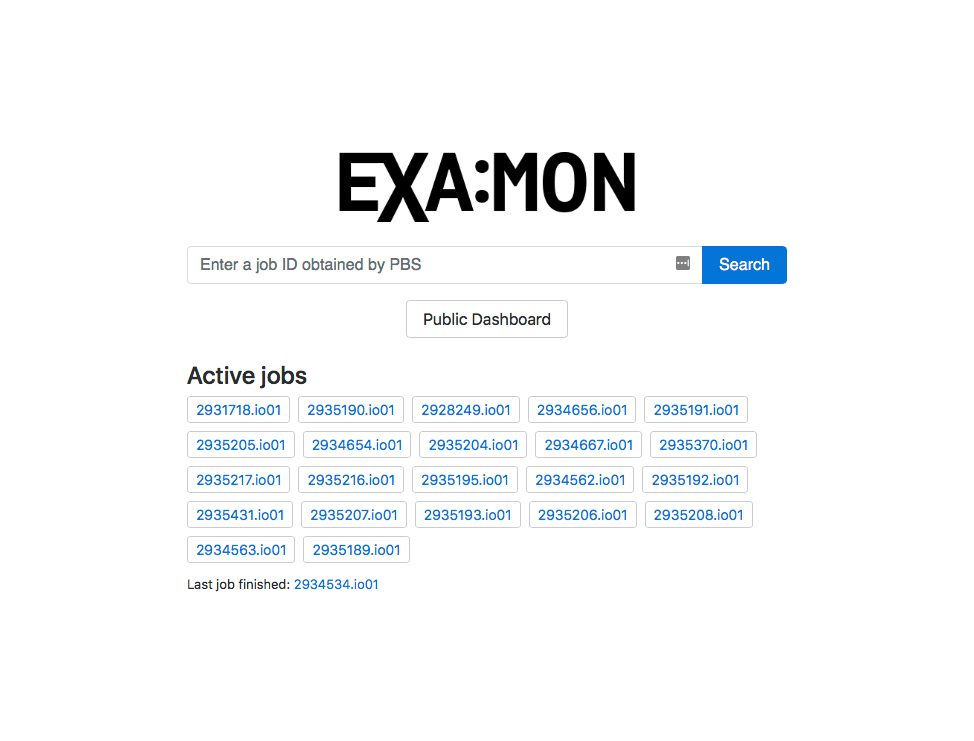
\includegraphics[width=\columnwidth]{job-lookup}
    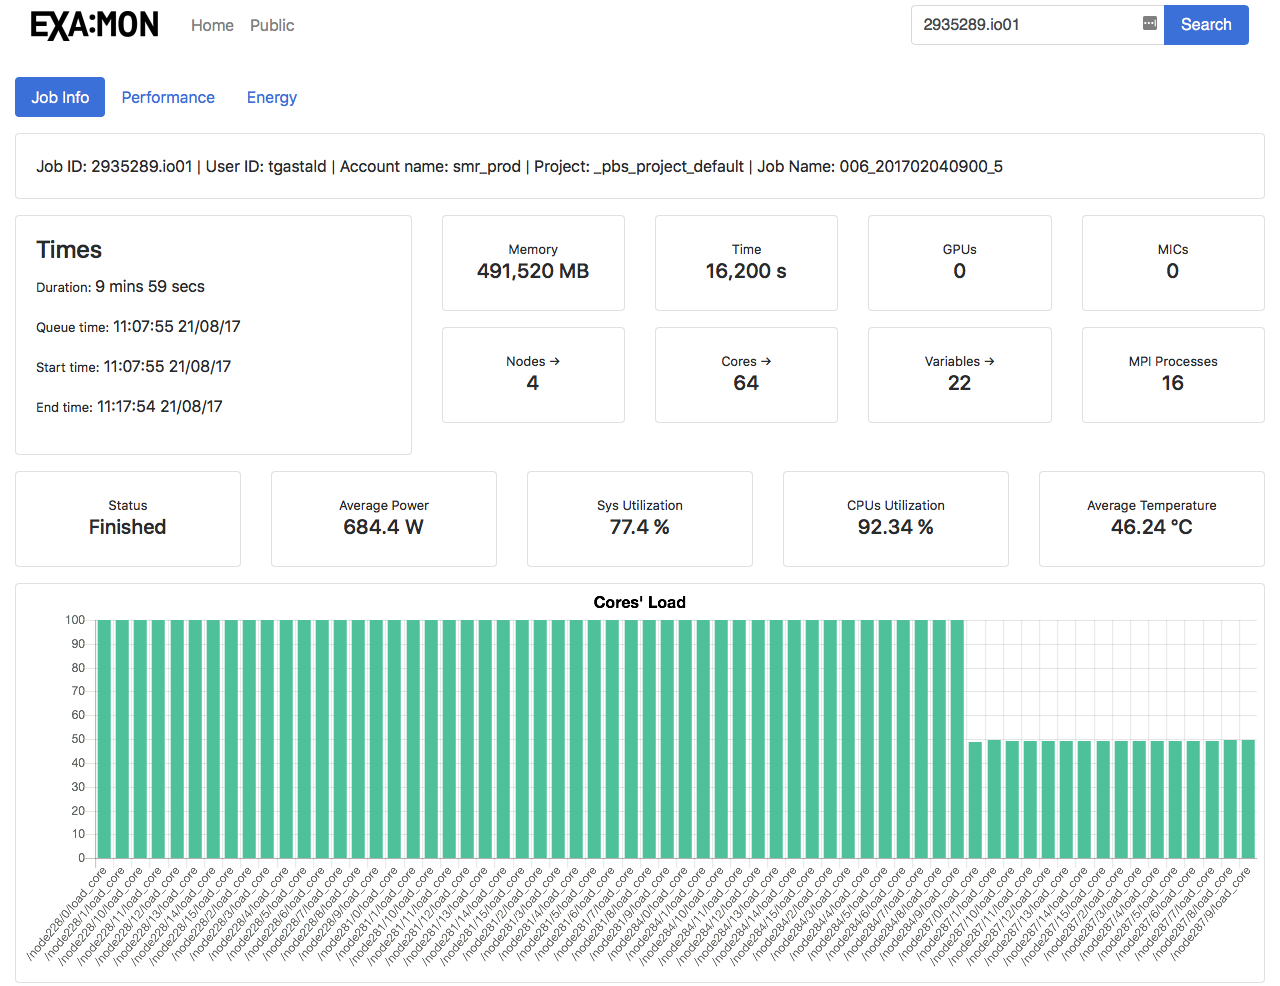
\includegraphics[width=\columnwidth]{job-info}
    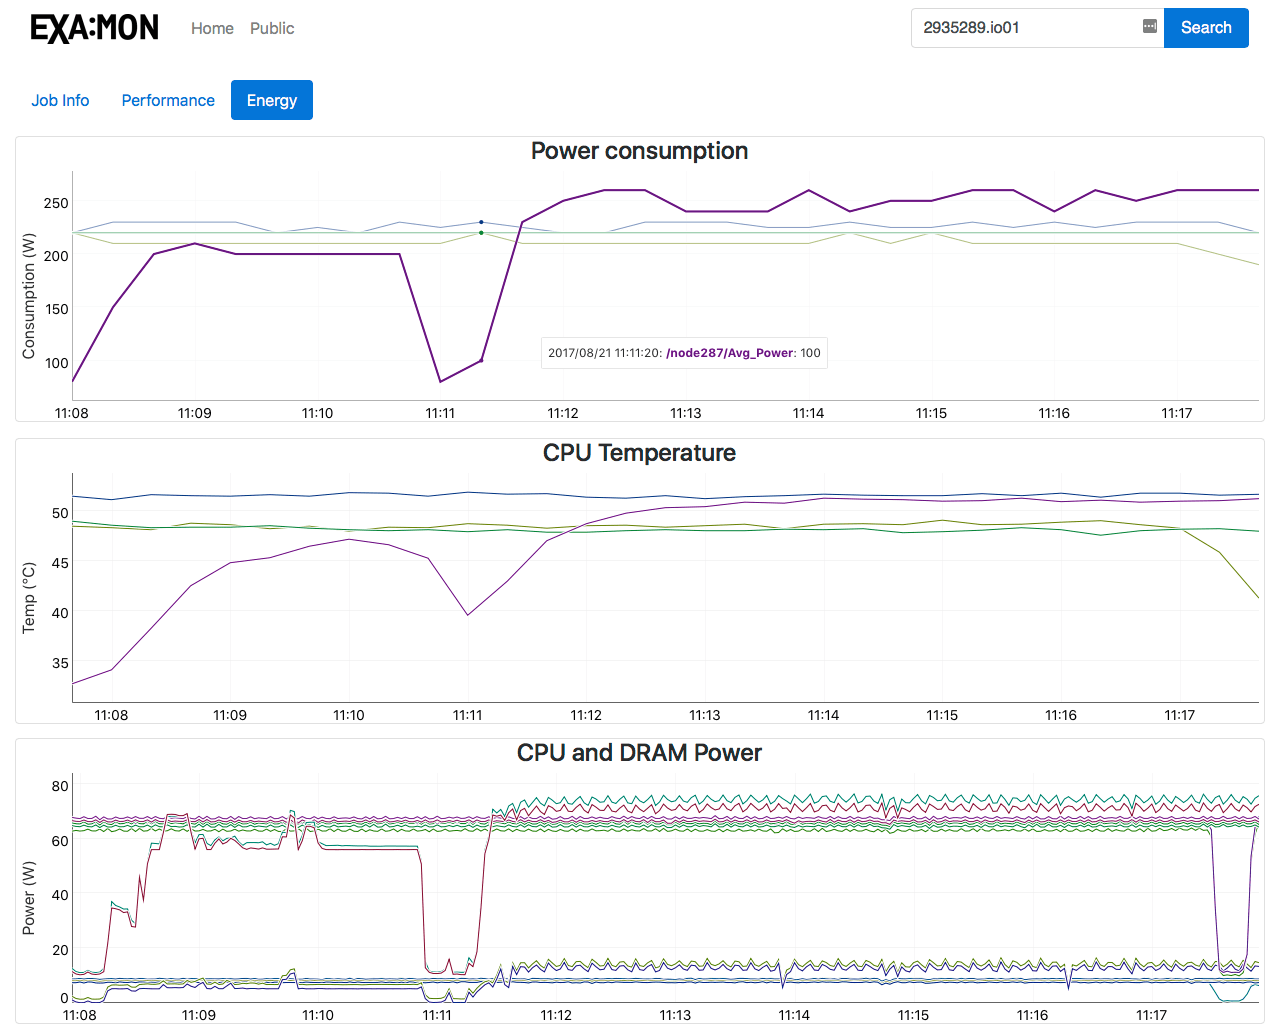
\includegraphics[width=\columnwidth]{job-energy}
    \caption{From left to right: intro page with jobs lookup, currently running jobs and last finished job; job's info dashboard with a finished job; job's energy dashboard.}
    \label{fig:job}
\end{figure*}

\section*{Methods}
The whole project can be separated into three phases. First phase is data anylysis where the whole dataset of available metrics was presented, how they are distributed and eventually processed on the back-end.

\itempar{Data Analysis}
Datasets can be divided into multiple levels of aggregation:
\begin{itemize}
    \item{Per-core level -- the most low-level data can be found in core's registers such as IPS, Lx-cache misses and more. It also provides info about its load and temperature.}
    \item{Per-CPU level -- each node consists of two CPUs and each of them can provide data about its C-states, energy counters and its frequency.}
    \item{Per-node level -- most of the information available on node-level basis are coming from IPMI\cite{ipmi}. Via this interface we can access info about node's utilization, multiple temperature sensors and average power consumption.}
    \item{Per-cluster level -- the Galileo's cluster room was equipped with several environmental sensors. This dataset is not currently available due to technical problems.}
    \item{Per-job level -- data gathered using the PBS scheduler's hooks. This dataset is aside from previous ones since it points to allocated and used resources of the job submitted to the queue. This data are stored directly to Cassandra cluster ommitting KairosDB.}
\end{itemize}

With each level we can aggregate the lower levels (except job-level data). This is especially useful for core-level data which are mostly too dense for any comprehensible visualisation.

\itempar{Visualisation}
Second phase was to visualize data stored in KairosDB in simple yet insightful way in a lightweight web application. The application, called ExaMon Web, uses Angular framework as its base on top of which several other libraries were used. Worth mentioning are Dygraphs and Bootstrap. The former library produces powerful time-oriented charts utilizing the canvas element in web browser. The latter is a CSS framework to produce uniform user interface across the whole application.

Compared to Grafana, the created web application feels more lightweight, fast and easier to use because of the prepared datasets which are being used. The balance between configurability and the ease of use must have been found. We concluded the best way to achieve this was to enable time selection on given datasets but restrict configurability of the charts themselves. This way user is not bogged down with configuration and only focuses on prepared data.

If there is such desire to see other metrics the Grafana framework is still available right next to the ExaMon Web. As an additional feature, compared to Grafana, we can perform more advanced queries using the KairosDB REST API.

\itempar{Live Data}
The last phase was to utilize the live stream of MQTT messages right in the ExaMon Web. Two use-cases were defined for the MQTT messages depending on their origin.

Several job info MQTT messages are send during the job's lifecycle inside the PBS and every job is assigned a unique job ID. Using the ID user can subscribe to given messages and view various information on the ExaMon Web job dashboard. The dashboard also uses Cassandra cluster in case the job is already finished and stored in the cluster. This way user can see additional data about their job.

Using the job data a user can view detailed info about allocated resources of the given job such as CPU load, system utilization and more as seen in \ref{fig:job}. With this information the user can asses some conclusions about their program. How effective it is, where are the slow parts and even perform a top-down analysis for performance issues. Also they can view how the program performed in terms of energy efficiency.

Second use-case is designed for general public and partly for system administrator. The use case is separated into two different parts. First one is very similar to job dashboards where data are displayed as time-serie charts with the difference in aggregation level which is at the cluster level. This means we can easily display, for example, the cluster's CPU load.

The other part is the most crucial in terms of interactive data visualisation. An accurate 3D model of the Galileo cluster was created using Blender and with the help of Blend4Web incorporated into the ExaMon Web. Even further, deeper integration was realized utilizing WebSockets (using Socket.io library) that enables us to create a reactive paradigm model instead of polling-based one. The model inside the page receives live data that has been published by the nodes and send to the broker. A subscription model was developed to accomodate large amount of visitors. The model then colours each node based on the minimum and maximum value of all received data. Weighted moving average was used in order to accomodate for sudden spikes in data using the given formula:

$v_{new} = v_{current} + v_{previous} \times (1 - \alpha)$

\noindent where $v_{previous}$ value is set to the first available value and $\alpha = 0.75$ as a default value was chosen based on short-term evaluation.

\section*{Results}

The web application ExaMon Web is ready for production and is already running on one of CINECA's virtual machine in staging environment. ExaMon Web can be split to two major parts: 1. Tool for overseeing job submitted to PBS queue. 2. Cluster-level visualisation and analysis.

We will describe both parts of the ExaMon Web with a prepared use-case scenario which were created during development.

\itempar{Job Visualiser}

\itempar{Cluster Visualiser}

\section*{Discussion \& Conclusion}


%\itempar{Introduction -- What is the project?}%
%The introduction should describe the question/problem/research area addressed by the project and set the context for your work. It should explain why your project is interesting or important. It should introduce the techniques and approach you used to complete the project.
%
%\itempar{Methods -- How did I complete the project?}%
%Briefly describe what was actually done. This should include more detail on techniques and approaches, with enough detail that an interested person could attempt to reproduce your work (You do not have to include every detail, but use citations to give the required background). 
%
%\itempar{Results -- What did I find out?}%
%Focus on what worked! Outline the outcomes and results of your project
%
%\itempar{Discussion \& Conclusion}
%(What does that mean?) Explain your conclusions and your interpretation of your results. How did it compare to what was to be expected or previous work? What implications does this have for other work?
%

\begin{figure*}[t!]
    %\color{yellow}\rule{2\columnwidth+\columnsep}{10cm}%
    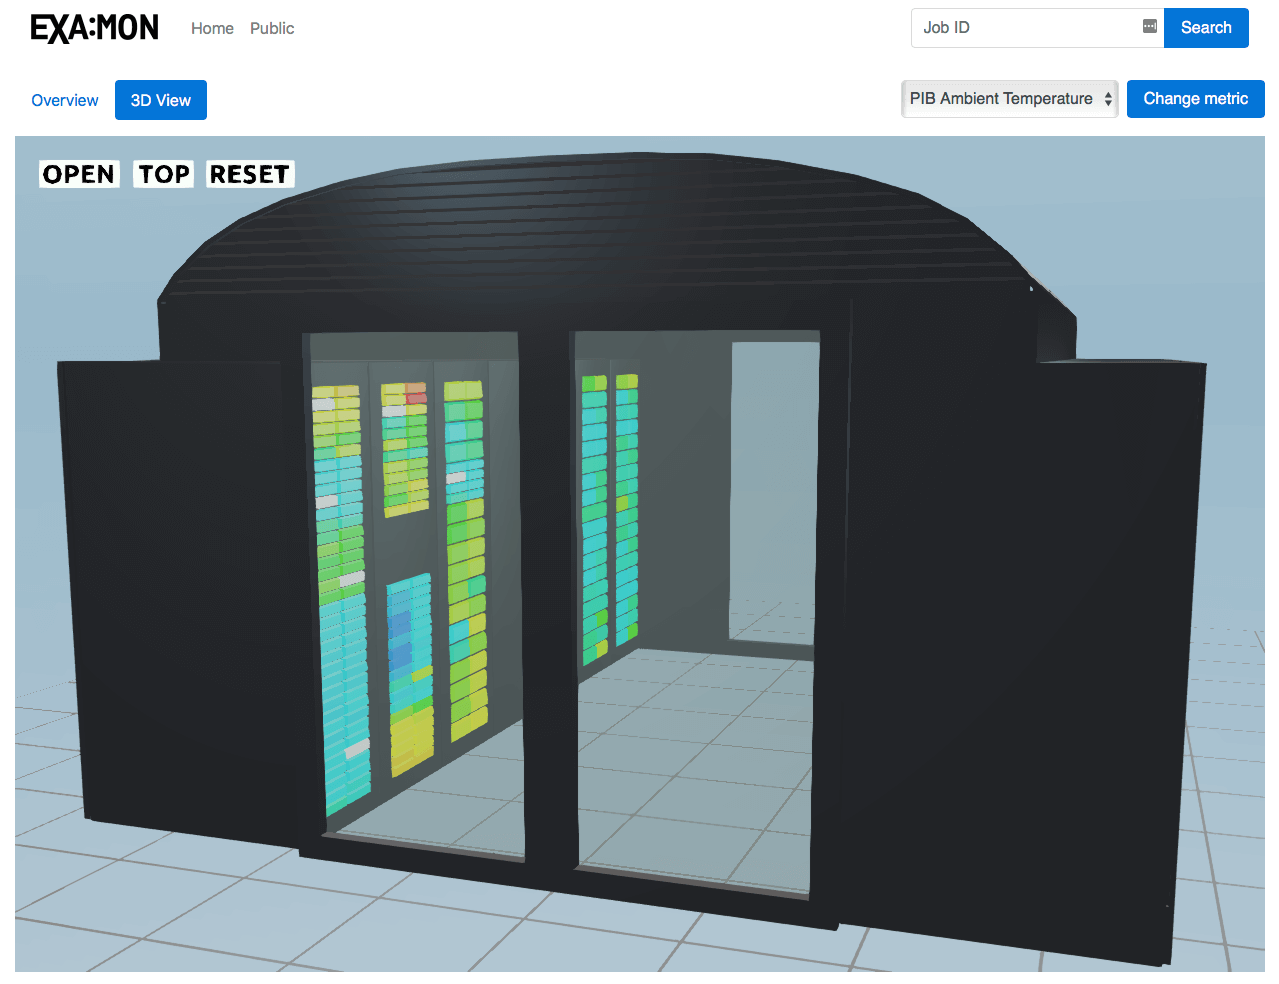
\includegraphics[width=2\columnwidth+\columnsep]{public-3d}
    \hspace{\columnsep}
    \begin{minipage}[b]{\columnwidth}
        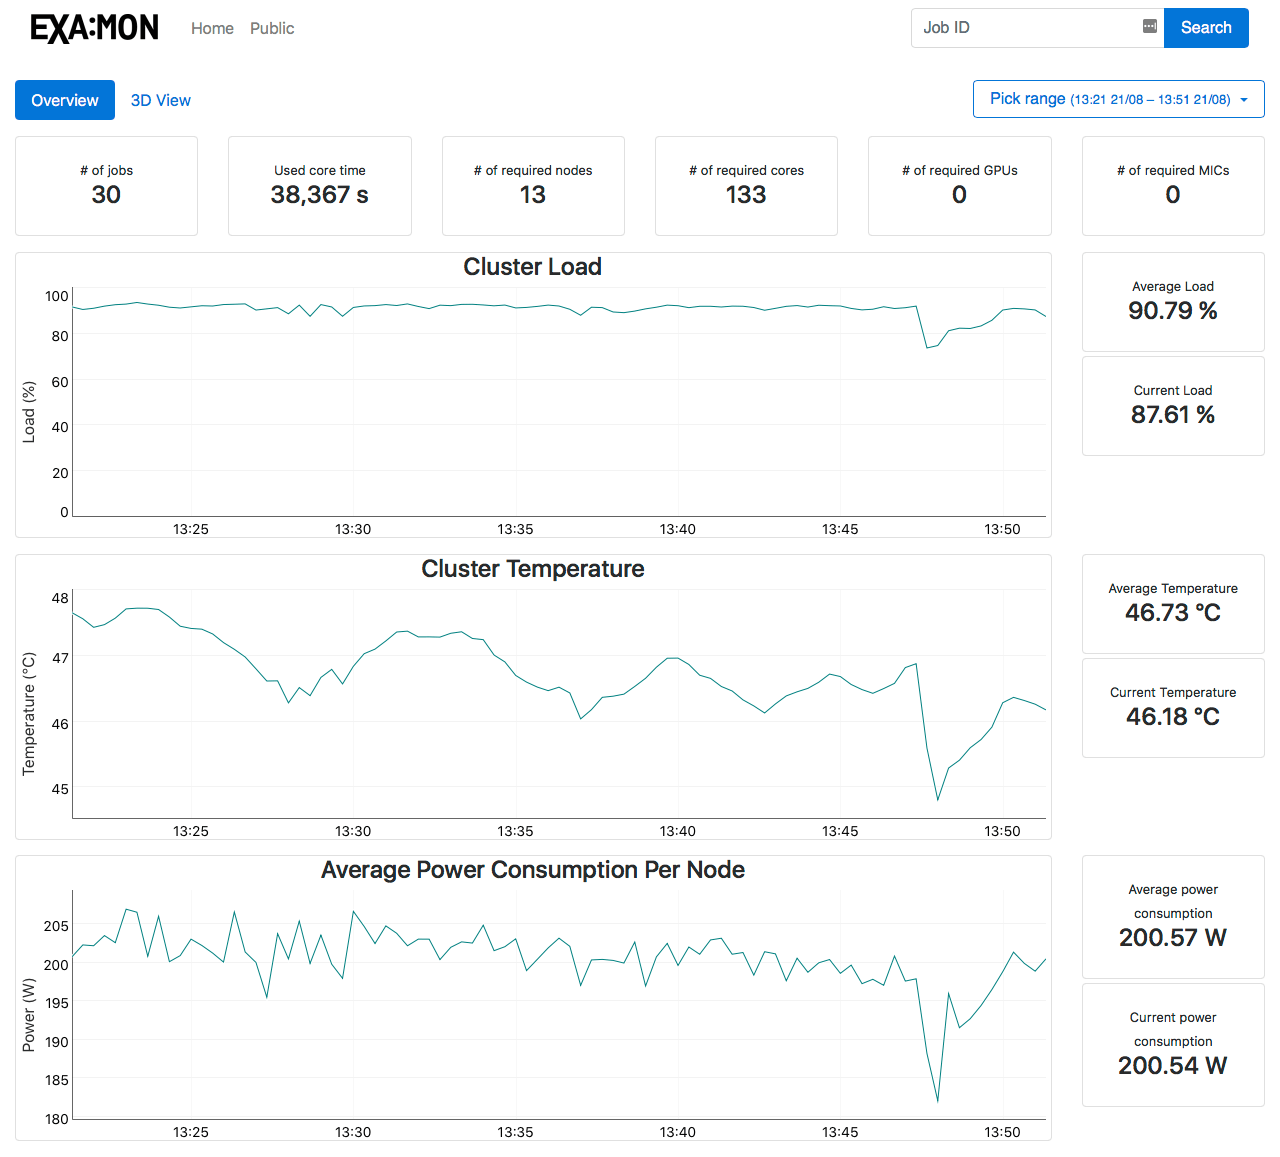
\includegraphics[width=\linewidth]{public-overview}
        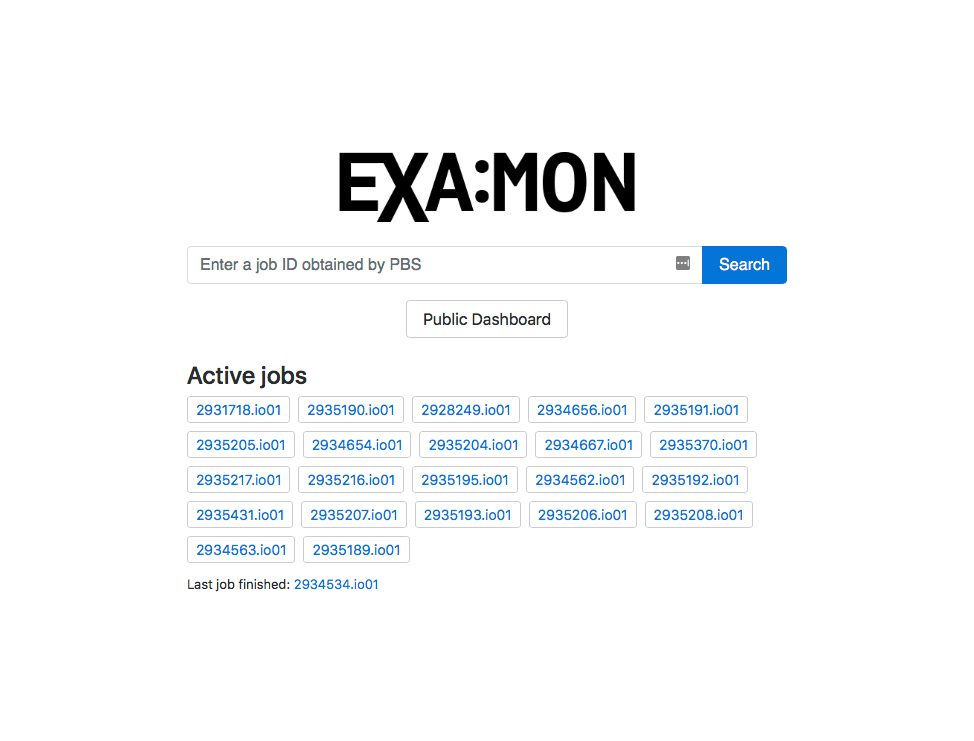
\includegraphics[width=\linewidth]{job-lookup}
    \end{minipage}
    \caption*{3D model}
    \label{fig:3d}
\end{figure*}

\itempar{Acknowledgements} (who helped me?) PRACE acknowledgement will be given together at the colophon. Site acknowledgement if required. Other acknowledgement if requested.

\newcommand{\sohpcinfo}[1]{\par\vspace{1ex}\footnotesize
  \textcolor{prace-lightblue}{PRACE SoHPC }%
  \textcolor{prace-darkblue}{#1}\\[0.5ex]\scriptsize
}

\renewcommand\refname{\usefont{OT1}{phv}{m}{n}\selectfont\small{References}}
\begin{thebibliography}{9}
\vspace*{-1ex}  % adjust this
\scriptsize
\bibitem[1]{current}
Beneventi, Francesco, et al. "Continuous learning of HPC infrastructure models using big data analytics and in-memory processing tools." 2017 Design, Automation \& Test in Europe Conference \& Exhibition (DATE). IEEE, 2017.

\bibitem[2]{mqtt}
Locke, Dave. "Mq telemetry transport (mqtt) v3.1 protocol specification." IBM developerWorks Technical Library (2010).

\bibitem[3]{kairos}
Goldschmidt, Thomas, et al. "Scalability and robustness of time-series databases for cloud-native monitoring of industrial processes." Cloud Computing (CLOUD), 2014 IEEE 7th International Conference on. IEEE, 2014.

\bibitem[4]{ipmi}
Kaufman, Gerald J. "System and method for application programming interface for extended intelligent platform management." U.S. Patent No. 7,966,389. 21 Jun. 2011.
APA
\end{thebibliography}

\vfill
\noindent\begin{minipage}[b]{0.7\linewidth}
\begin{flushleft}
  \usefont{OT1}{phv}{m}{n}\selectfont
  \sohpcinfo{Project Title}
  \href{https://summerofhpc.prace-ri.eu/web-visualization-of-energy-load-of-an-hpc-system/}{Web visualization of Energy load of an HPC system}
  
  \sohpcinfo{Site}
  CINECA, Italy
  
  \sohpcinfo{Authors}
  \href{mailto:xstehl14@stud.fit.vutbr.cz}{\theauthor},
  BUT, Czech Republic
  
  \sohpcinfo{Mentor}
  \href{mailto:a.bartolini@unibo.it}{Dr. Andrea Bartolini}, UNIBO, Italy
\end{flushleft}
\end{minipage}\hfill%
\begin{minipage}[b]{0.3\linewidth}
  \color{prace-darkblue}\rule{\linewidth}{2.5cm}\par
  \tiny\theauthor
\end{minipage}%
\vspace{-1.5ex}% any of information below is optional
\begin{flushleft}
  \sohpcinfo{ More Information}
  \href{https://www.angular.io}{Angular} \\
  \href{http://dygraphs.com}{Dygraphs}  \\
  \href{http://getbootstrap.com}{Bootstrap} \\
  \href{https://www.blender.org}{Blender} \\
  \href{https://www.blend4web.com/en/}{Blend4Web}

\sohpcinfo{ Acknowledgement}
Write any requested acknowledgements or thanks here. Mentors should be
asked for them too.

\sohpcinfo{ Project ID} 1705

\end{flushleft}
\end{multicols}
\end{document}

%%Local Variables:
%%% mode: latex
%%% TeX-parse-self: t
%%% TeX-auto-save: t
%%% TeX-source-specials-mode: t
%%% TeX-PDF-mode: t
%%% LaTeX-command: "pdflatex -synctex=1  --enable-write1"
%%% TeX-master: t
%%% ispell-local-dictionary: "british"
%%% End:

